\documentclass{beamer}
\newcommand\measurepage{\dimexpr\pagegoal-\pagetotal-\baselineskip\relax}
\title{Team W - Algorithms for Sports Eliminations}
\author{
    Gordon Reid: 1002536R\\
    Ryan Wells: 1002253W\\
    Kris Stewart: 1007175S\\
    David Selkirk: 1003646S\\
    James Gallagher: 0800899G\\
    Dr David Manlove: Project Supervisor
}
\date{March 19, 2013}
\begin{document}
\frame{\titlepage}
%"Presentations should describe the aims and objectives of the project, the
%work you have undertaken and the resulting product, the key design and
%management decisions you made, and any lessons learnt. Tell us what you’ve
%done, why it was interesting, what you learnt, what you’d do differently if you
%had to do it again, etc."

% introduction - Ryan - 2 minutes (2)
% Parser - Kris - 5 minutes (7)
% Desktop UI - David - 5 minutes (12)
% Web UI - Gordon - 3 minutes (15)
% Algorithm - Ryan - 3 minutes (18)
% User Eval - James - 5 minutes (23)
% Conclusion - Gordon - 2 minutes (25)
\frame{
  \frametitle{Project introduction}
  \begin{itemize}
  \item Project aims to answer sports elimination question.
  \item What is sports elimination?
  \item Main modules: Parsing, Desktop/Web User Interface, Algorithm, User Evaluation
  \item Builds on na\"{\i}ve calculations made by sports pundits.
  \end{itemize}
}
\frame{
  \frametitle{Sport}
  \begin{itemize}
  \item American Major League Baseball.
  \item 1 point for a win, 0 points for a loss, no draws allowed.
  \item 2012 season ran from 5th April to 4th October.
  \item Six divisions with four to six teams per division.
  \end{itemize}
}
\frame{
  \frametitle{Example}
  \begin{center}
  \begin{figure}
  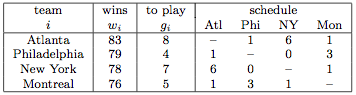
\includegraphics[width=\textwidth]{Example.png}
  \end{figure}
  \tiny{Image courtesy of Kevin D. Wayne, Princeton University}
  \end{center}
  \begin{itemize}
  \item Montreal trivially eliminated
  \item Philadelphia non-trivially eliminated
  \end{itemize}
}
\frame{
\frametitle{Parser}
\pause
\begin{center}
\begin{figure}
%can you make the image the sample one used in the dissertation with 2 dates shown
%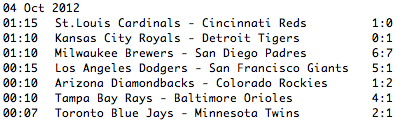
\includegraphics[width=\textwidth]{textfile.png}
\end{figure}
\end{center}
\begin{itemize}
\item Retrospective real world data instead of hard coding
\item Source file sample
\item Generate your own
\end{itemize}
}
\frame{
\frametitle{Parser}
\begin{itemize}
\item 3 main objects of the application
\item[Division] Teams of division, matches to be played, if they've been played
\item[Match] Team names, scores, if it's been played
\item[Team] Team name, points in league, eliminated status
\item Date emulation
\item Had considered future plans to parse a web page.
\item As a team we decided not to implement and focus on other avenues
\end{itemize}
}
\frame{
  \frametitle{User Interface}
  % Show file menu
  % Talk about Java Swing
  \begin{itemize}
  \item User is likely an advanced follower of the sport looking for
  very specific information.
  \item Simple design based on presenting this key information immediately.
  \item More detailed information available on user request.
  \item Written in Java Swing. Netbeans was considered, but dropped.
  \end{itemize}
}
\frame{
  \frametitle{User Interface - Key Tasks}
  \begin{itemize}
  \item Display all teams by division and league, showing elimination status.
  \item Update the elimination status on start-up.
  \item Display certification of elimination for teams eliminated.
  \end{itemize}
}
\frame{
  \frametitle{User Interface - Prototype}
  \begin{figure}
  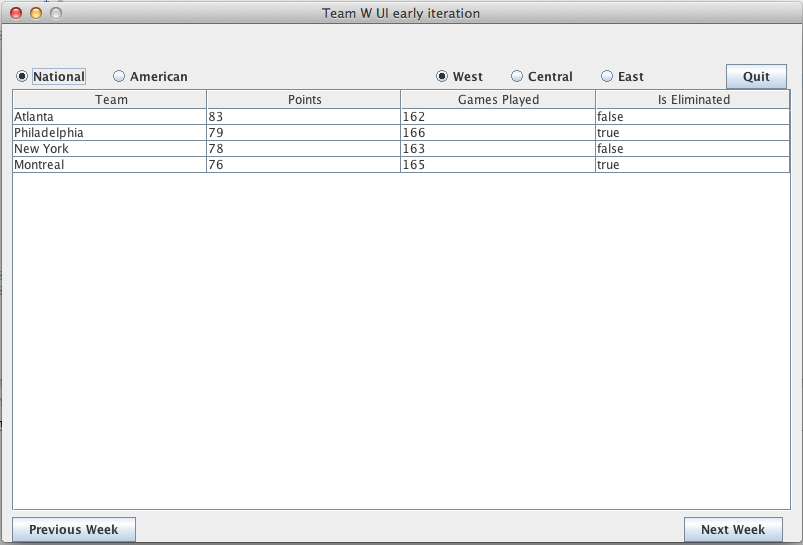
\includegraphics[width=\textwidth]{InitialUI.png}
  \begin{itemize}
  \item Written in Java Swing. Netbeans was considered, but after
  some experimentation was dropped.
  \end{itemize}
  \end{figure}
}
\frame{
  \frametitle{User Interface - Additional Tasks}
  \begin{itemize}
  \item Allow date navigation, displaying correct results for each the date.
  \item Display print functionality.
  \item Display league generation functionality.
  \end{itemize}
}
\frame{
  \frametitle{User Interface - Final}
  \begin{figure}
  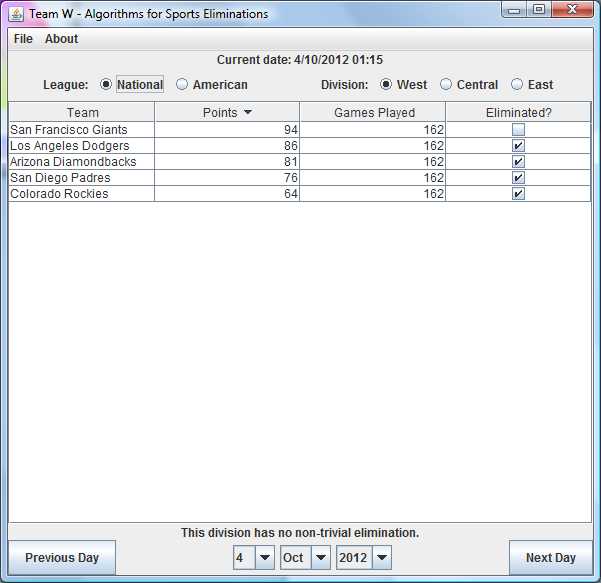
\includegraphics[scale=0.4,keepaspectratio]
  {finalDesktopUI.png}
  \end{figure}
}
\frame{
  \frametitle{User Interface - Final}
  \begin{figure}
  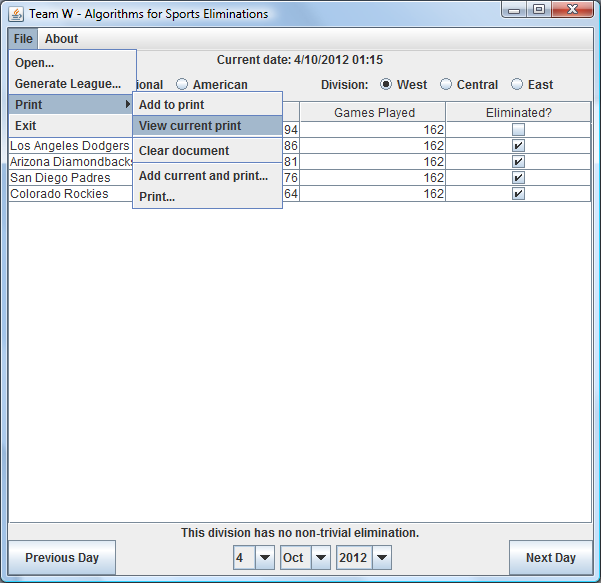
\includegraphics[scale=0.4,keepaspectratio]
  {UIFileMenu.png}
  \end{figure}
}
\frame {
  \frametitle{Web Application}
  \begin{itemize}
  \item<2-> An extension of the project.
  \item<2-> Contains a subset of most important functionality of
  desktop application.
  \item<2-> Uses multiple technologies including HTML, CSS, JS, PHP, jQuery.
  \item<2-> Tested on all major browsers for compatibility.
  \item<2-> Numerous extensions of web application part of future work.
  \end{itemize}
}
\frame {
  \frametitle{Web Application Screenshot}
  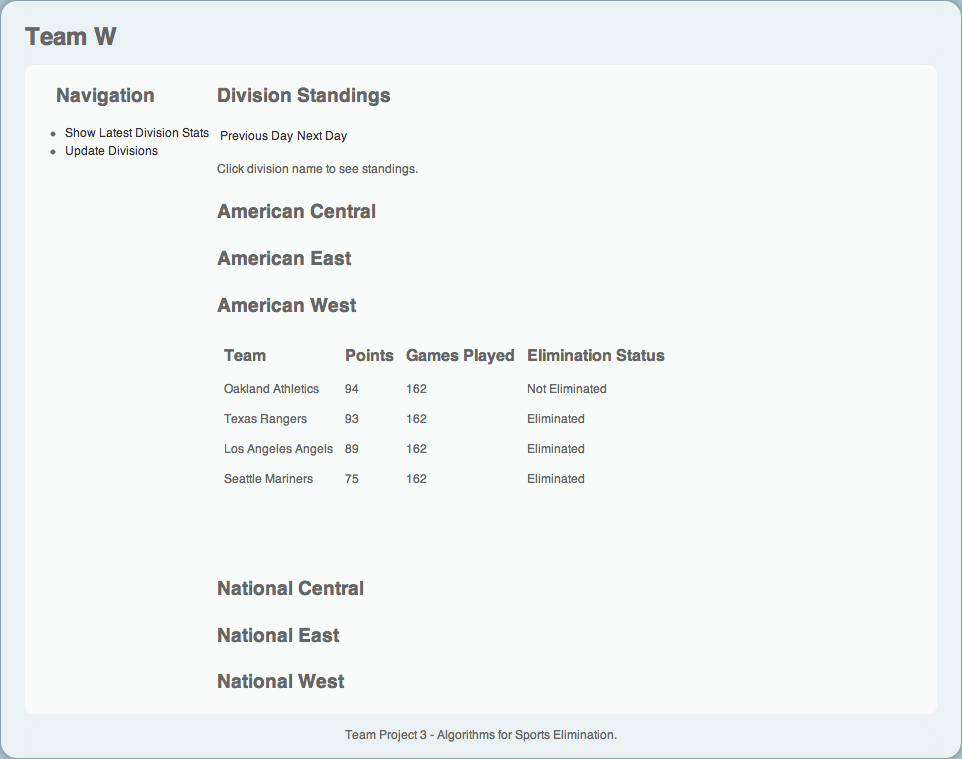
\includegraphics[width=\textwidth,height=\measurepage,keepaspectratio]
  {webAppScreenshot.png}
}
\frame{
  \frametitle{Algorithm}
% Remaining schedule of games
% Clarify saturating flow and meaning of elimination.
% Safe to NOT mention augmenting paths.
% Tie up network flow to elimination problem.
% Non-trivial elimination is what FF is for
  \pause
  \begin{itemize}
  \item<2-> Revolves around creation of directed graphs and flow
    through directed graphs.
  \item<3-> Pushing flow through a specific graph will allow us to
    determine if the given team X is eliminated from a given league.
  \item<4-> A team X can win the league if it is possible for there to
    be a saturating flow. A flow is saturated if the total flow from
    the source equals the total capacity from the source.
  \item<5-> All flow leaving the source has to arrive at the sink.
  \end{itemize}
}
\frame{
  \frametitle{Algorithm - Graph}
  \begin{center}
  \begin{figure}
  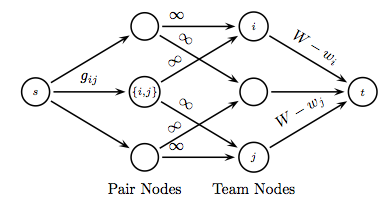
\includegraphics[width=0.6\textwidth]{graph.png}
  \end{figure}
  \tiny{Image courtesy of Kevin D. Wayne, Princeton University}
  \end{center}
  \begin{itemize}
  \item $team_k$ - Team being tested for elimination.
  \item $team_i$ and $team_j$ - Arbitrary teams in $team_k$'s division
  \item $g_{i, j}$ - Number of games left between $team_i$ and $team_j$
  \item W - Current score of $team_k$ + games $team_k$ has remaining
  \item $w_{i}$ - Number of game $team_i$ won
  \end{itemize}
}
\frame{
  \frametitle{Algorithm - Extensions}
  \begin{itemize}
    \item<2-> League Elimination by Binary Search Computation % Clarify
    \item<3-> Certificate of Elimination
    \item<4-> First non-trivially eliminated team % Clarify
  \end{itemize}
}
\frame {
\frametitle{User Evaluation}
Aim : Gain quality feedback regarding the usability of the system we created.

Structure :
\begin{itemize}
\item<1->Stage 1 : Participant Brief. ( Intro )
\item<2->Stage 2 : Task Script ( Usability )
\item<3->Stage 3 : Questionnaire ( Likeability )
\end{itemize}
}
\frame{
\frametitle{Surprises!}
Lots of interesting lessons learned!
\begin{itemize}
\item<1-> Gained tangible results very quickly.
\item<2-> Design faults tripped up even the most experienced of users.
\item<3->Very wide variety of attention span in test group.
\item<4-> User's got tripped up by testing method.
\end{itemize}
}
\frame{
\frametitle{Varied and Quality Feedback: Examples }
Overall User Evaluation was very successful.

Gained a diverse range of quality feedback from test subjects.

Discovered Bugs, Usability Issues and Design Flaws.
\begin{itemize}
\item<1-> Design Flaws : Radio Button for League and Division selection.
\item<2->Usability Issues : Inadequate Documentation provided at time of testing/
Missed Functionality !
\item<3-> Bugs : Date not being displayed on loading
of Web application.
\end{itemize}
}
\frame{
\frametitle{Over Very Positive Feedback!}
System received numerous positive comments on usability and aesthetic.
\begin{itemize}
\item<1-> Diverse range of feedback gained highlighted value of thorough user testing.
\item<2-> Provided great ideas for future work, design improvements, tweaks etcetera.
\item<3-> Lots of users interested in the system, even if had no interest in the domain.
\end{itemize}
}
\frame {
  \frametitle{Lessons Learnt and Future Work}
  Lessons Learnt
  \begin{itemize}
  \item Communication - Keep it simple.
  \item Leadership - May be required.
  \item Time management on a larger scale.
  \end{itemize}
  Future Work
  \begin{itemize}
  \item Complete changes suggested based on user evaluation.
  \item Continue implementation of web application.
  \item Binary first non-trivial elimination search.
  \end{itemize}
}
\frame {
  \frametitle{Project Conclusion}
  \begin{itemize}
  \item Successfully implemented all must have functionality.
  \item Fun and interesting to take theory and implement real-world application.
  \item Informative user evaluation.
  \item Plenty of scope for future work.
  \end{itemize}
}
\frame {
  We would now like to invite questions from the panel.

  Thank you for listening.
}
\end{document}
